\documentclass[11pt]{article}
\usepackage[T1]{fontenc}
\usepackage{amsmath,amssymb}
\usepackage{hyperref}
\usepackage{bookmark}
\usepackage{enumitem}
\usepackage{geometry}
\usepackage[many]{tcolorbox}
\geometry{margin=2.5cm}
% chktex-file 26
% chktex-file 13
\usepackage{tikz}
\usetikzlibrary{trees}


\tcbset{
  mydefstyle/.style={
    colback=white,
    colframe=black,
    fonttitle=\bfseries,
    boxrule=0.8pt,
    arc=4pt,
    left=3mm, right=3mm, top=2mm, bottom=2mm,
    breakable
  }
}

% Environnement "définition encadrée"
\newtcolorbox{defbox}[2][]{mydefstyle,title=#2,#1}

\title{Constrained Pseudorandom Functions, Revisited}
\author{\textbf{Julian Mouthon, Mario Razafinony}}
\date{\today}

\usepackage{fancyhdr}
\setlength{\headheight}{13.59999pt}
\pagestyle{fancy}

\fancyhf{}

\fancyhead[L]{Constrained Pseudorandom Functions, Revisited}
\fancyhead[R]{Sorbonne Université}
\fancyfoot[C]{\thepage}


\begin{document}

\begin{figure}
  \centering
  \includegraphics[width=0.4\textwidth]{./images/sorbonne.png}
\end{figure}


\maketitle

\section*{Introduction}

Ce projet s’inscrit dans le cadre de l’étude des fonctions pseudo-aléatoires contraintes
(\emph{Constrained Pseudorandom Functions}, CPRF), une extension des fonctions
pseudo-aléatoires classiques permettant de restreindre les évaluations à un sous-ensemble
d’entrées défini par une contrainte.

Dans un premier temps, nous présentons les notions fondamentales liées aux fonctions
pseudo-aléatoires et aux CPRFs, ainsi que la construction proposée par Bost, Minaud et
Ohrimenko en 2017 (BMO17).

Dans un second temps, nous nous intéressons aux travaux récents de Cheng et Jaeger
en 2025 (CJ25), qui mettent en évidence une attaque contre cette CPRF et proposent une variante
hachée assurant la sécurité dans un nouveau modèle. 

\newpage

\tableofcontents
\newpage

\section{Définitions}

\addcontentsline{toc}{subsection}{Fonction pseudo-aléatoire}
\begin{defbox}{Fonction pseudo-aléatoire (PRF)}

Une fonction pseudo-aléatoire
\[
F : \mathcal K \times D \rightarrow R
\]
est une fonction telle que, pour une clé secrète $K$, la fonction $F(K,\cdot)$ est
indiscernable d’une fonction réellement aléatoire
$G : D \rightarrow R$ pour tout adversaire efficace.
\end{defbox}

\addcontentsline{toc}{subsection}{Contrainte}
\begin{defbox}{Contrainte}

Une contrainte est un prédicat booléen
\[
C : D \rightarrow \{0,1\},
\]
qui partitionne le domaine $D$ en deux ensembles:
\begin{itemize}
\item les entrées \emph{autorisées}, telles que $C(x)=1$
\item les entrées \emph{interdites} (ou contraintes), telles que $C(x)=0$
\end{itemize}

Intuitivement, la contrainte spécifie l’ensemble des entrées sur lesquelles une clé
contrainte est autorisée à évaluer la fonction pseudo-aléatoire.

Ici, nous considérons principalement des contraintes de la forme
\[
C_n(x) = [x < n],
\]
qui autorisent toutes les entrées strictement inférieures à un seuil $n \in \mathbb{N}$.
\end{defbox}

\addcontentsline{toc}{subsection}{Fonction pseudo-aléatoire contrainte}
\begin{defbox}{Fonction pseudo-aléatoire contrainte (CPRF)}
Une fonction pseudo-aléatoire contrainte (CPRF) est donnée par quatre algorithmes efficaces:
\begin{itemize}
\item $\textsf{Setup}(1^\lambda) \to K$ (clé maître): génère la clé secrète principale $K$.
\item $\textsf{Constrain}(K,C) \to K_C$ (clé contrainte): produit une clé spéciale $K_C$ permettant
d’évaluer la fonction uniquement sur les entrées autorisées par $C$.
\item $\textsf{Eval}(K,x) \to y$ : évalue la fonction pseudo-aléatoire sur une entrée $x$ avec la clé maître.
\item $\textsf{EvalC}(K_C,x) \to y$ : évalue la fonction sur l’entrée $x$ avec la clé contrainte $K_C$.
\end{itemize}

Une CPRF est correcte si, pour toute clé $K$, toute contrainte $C$ et toute entrée $x$
telle que $C(x)=1$, on a
\[
\textsf{EvalC}(K_C,x)=\textsf{Eval}(K,x).
\]

Autrement dit, la clé contrainte permet d’évaluer la PRF exactement sur les entrées autorisées.
\end{defbox}

\section{Construction de la CPRF de BMO17}

\subsection{Propriétés}

La CPRF de BMO17 est basée sur l'itération successive d'une permutation à trappe,
c’est-à-dire une fonction bijective facile à calculer mais difficile à inverser sans information secrète.
On note cette permutation $\pi$.

\addcontentsline{toc}{subsubsection}{Clé maîtresse}
\begin{defbox}{Génération de la clé maîtresse}
La clé maîtresse est composée des éléments suivants :
\begin{itemize}
  \item $ST_0 \in \mathbb{Z}_N$, un état initial secret choisi aléatoirement
  \item $SK$, une clé secrète RSA définissant la permutation à trappe $\pi_{SK}$
\end{itemize}
La clé publique associée $PK$ permet uniquement de calculer la permutation directe $\pi$.
\end{defbox}

\addcontentsline{toc}{subsubsection}{Evaluation avec clé maîtresse}
\begin{defbox}{Evaluation de la CPRF avec la clé maîtresse}
    
Avec la clé maîtresse $(ST_0, SK)$ et une entrée $c$, on peut évaluer la CPRF sur $c$ par :
\[
Eval((SK, ST_0), c) = \pi_{SK}^{-c}(ST_0)
\]

L’évaluation consiste à appliquer $c$ fois l’inverse de la permutation à partir de l’état initial $ST_0$.
\end{defbox}

\addcontentsline{toc}{subsubsection}{Clé contrainte}
\begin{defbox}{Génération de la clé contrainte}
À partir de la clé maîtresse $(ST_0, SK)$ et d’un entier $n$, correspondant à la contrainte
$C(c) = [c < n]$, la clé contrainte est composée des éléments suivants :
\begin{itemize}
  \item $PK$, la clé publique associée à la permutation $\pi$
  \item $ST_n = \pi_{SK}^{-n}(ST_0)$
  \item $n$
\end{itemize}

La clé secrète $SK$ n’est pas incluse dans la clé contrainte.
\end{defbox}

\addcontentsline{toc}{subsubsection}{Évaluation avec clé contrainte}
\begin{defbox}{Évaluation de la CPRF avec la clé contrainte}
    
Avec la clé contrainte $(PK, ST_n, n)$ et une entrée $c$, l’évaluation est possible uniquement si
$c < n$.
Dans ce cas, la valeur de la CPRF est calculée comme suit :
\[
\textsf{EvalC}((PK, ST_n, n), c) = \pi_{PK}^{\,n-c}(ST_n)
\]

Cette valeur est égale à $Eval((SK, ST_0), c)$ par construction, ce qui assure la correction du schéma.
\end{defbox}



\subsection{Implémentation}

Nous utilisons la bibliothèque OpenSSL pour la gestion des grands entiers
(\texttt{BIGNUM}), les opérations modulaires et le calcul de hachage SHA-256.

L’aléa est sécurisé et est obtenu à partir de \texttt{/dev/urandom}, ce qui
permet de générer l’état initial $ST_0$ ainsi que les paramètres RSA de manière sûre.


\subsubsection{Permutation RSA}

La permutation à trappe utilisée dans BMO17 est défini à l’aide de RSA.
Nous implémentons la génération de clés RSA de taille 2048 bits, ainsi que l’évaluation
de la permutation dans les deux sens.

Plus précisément, la fonction publique correspond à:
\[
x \mapsto x^e \bmod N,
\]
tandis que l’inverse de la permutation est calculé via:
\[
x \mapsto x^d \bmod N.
\]

avec 

\[
x^{e \cdot d} = x \bmod N , \forall x \in \mathbb{Z}_N.
\] 

Afin de limiter les fuites par canaux auxiliaires, l’évaluation privée est réalisée à l’aide
de la fonction \texttt{BN\_mod\_exp\_mont\_consttime} d’OpenSSL, qui garantit un temps
d’exécution indépendant des données.


\subsubsection{Clé maîtresse}

La clé maîtresse de la CPRF est composée d’un état initial secret $ST_0$ et d’une clé
privée RSA. L’état initial est généré comme un entier aléatoire de 256 bits à partir de
\texttt{/dev/urandom}..

L’évaluation avec la clé maîtresse consiste à appliquer $c$ fois l’inverse de la permutation
RSA à partir de $ST_0$.

\subsubsection{Clé contrainte}

À partir de la clé maîtresse et d’un paramètre de contrainte $n$, nous dérivons une clé
contrainte composée de la clé publique RSA $(e, N)$ et de l’état
\[
ST_n = \pi^{-n}(ST_0).
\]

Cette clé permet ensuite d’évaluer la CPRF uniquement pour les entrées $c < n$ en
appliquant $(n-c)$ fois la permutation publique à partir de $ST_n$. La clé privée n’est
jamais incluse dans la clé contrainte, ce qui garantit que seules les évaluations autorisées
sont possibles.

\subsection{Tests d'amélioration}
\subsubsection{Permutation à trappe Rabin}

\paragraph{}La permutation de Rabin est une fonction cryptographique à trappe fondée sur la difficulté de la factorisation des entiers. Elle est conceptuellement plus simple que RSA et repose sur l'opération de mise au carré modulo un entier composé.

\begin{itemize}
\item\textbf{Génération de la clé :}

On choisit deux nombres premiers distincts $p$ et $q$ tels que :
\[
p \equiv q \equiv 3 \pmod{4}
\]

La clé publique est définie par :
\[
n = p \cdot q
\]

La clé privée est le couple $(p, q)$.

Cette condition sur $p$ et $q$ permet un calcul efficace des racines carrées modulo ces nombres premiers.

\item\textbf{Permutation de Rabin :}

La permutation de Rabin est la fonction :
\[
f : \mathbb{Z}_n \rightarrow \mathbb{Z}_n
\]
définie par :
\[
f(x) = x^2 \bmod n
\]

Cette fonction est facile à calculer, mais difficile à inverser sans connaître la factorisation de $n$.

\item\textbf{Inverser la permutation de Rabin :}

Inverser la permutation de Rabin revient à résoudre l'équation :
\[
x^2 \equiv y \pmod{n}
\]

Lorsque $n = p \cdot q$, cette équation admet exactement \textbf{quatre solutions distinctes} modulo $n$.

%\subsection{Résolution modulo p et q}

On commence par réduire le problème modulo $p$ et $q$ :
\[
\begin{cases}
x^2 \equiv y \pmod{p} \\
x^2 \equiv y \pmod{q}
\end{cases}
\]

Comme $p \equiv 3 \pmod{4}$, une racine carrée modulo $p$ est donnée par :
\[
r_p = y^{\frac{p+1}{4}} \bmod p
\]

De même, modulo $q$ :

\[
r_q = y^{\frac{q+1}{4}} \bmod q
\]

Les solutions sont donc: 

\begin{itemize}
  \item $X_0 = (r_p * q * q^{-1}_{\bmod p} + r_q * p * p^{-1}_{\bmod q}) \bmod n $

  \item $X_1 = (r_p * q * q^{-1}_{\bmod p} - r_q * p * p^{-1}_{\bmod q}) \bmod n$

  \item $X_2 = (-r_p * q * q^{-1}_{\bmod p} + r_q * p * p^{-1}_{\bmod q}) \bmod n$

  \item $X_3 = (-r_p * q * q^{-1}_{\bmod p} - r_q * p * p^{-1}_{\bmod q}) \bmod n$
\end{itemize}


\end{itemize}

\paragraph{Problème:}Laquelle de ces racines correspond au message original ?
\paragraph{}
La fonction \(f(x) = x^2 \bmod n\) n'est pas injective: chaque chiffré \(c\) a 4 pré-images.
Même avec la clé secrète (\(p,q\)), on peut calculer toutes les racines mais \textbf{pas déterminer directement celle qui correspond au message initial}.
Appliquer l'inverse \(n-c\) fois n'assure pas de retrouver le message original.



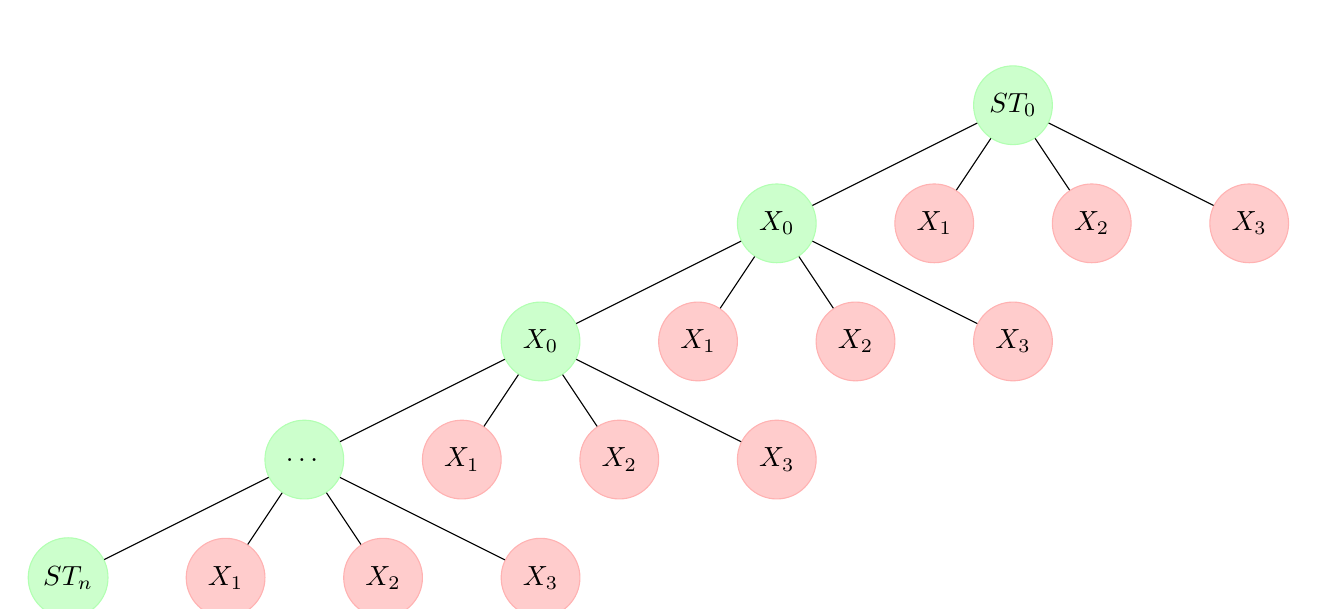
\begin{tikzpicture}[
  grow=down,
  sibling distance=20mm,
  level distance=15mm,
  every node/.style={fill=red!20,draw=red!30, circle, rounded corners, align=center, minimum width=10mm},
  correct/.style={draw=green!30, fill=green!20},
  level label/.style={font=\small, anchor=west, align=left}
]

\node[correct] {$ST_0$}
  % Niveau 1
  child {node[correct] {$X_0$} 
    % Niveau 2
    child {node[correct] {$X_0$} 
      % Niveau 3 
      child {node[correct] {$\dots$} 
        child {node[correct] {$ST_n$}}
        child {node {$X_1$}}
        child {node {$X_2$}}
        child {node {$X_3$}}
      }
      child {node {$X_1$}}
      child {node {$X_2$}}
      child {node {$X_3$}}
    }
    child {node {$X_1$}} 
    child {node {$X_2$}}
    child {node {$X_3$}}
  }
  child {node {$X_1$}} 
  child {node {$X_2$}}
  child {node {$X_3$}};
\end{tikzpicture}

\subsubsection{AES}
\paragraph{}
Le chiffrement AES applique une fonction bijective \(E_k(x)\) qui dépend de la clé \(k\).
Contrairement à \(x \mapsto x^2 \bmod n\), AES est injectif et chaque bloc chiffré a une \textbf{unique pré-image} pour une clé donnée.
Cependant, pour déchiffrer, il faut absolument connaître la clé \(k\) :
\begin{itemize}
    \item Sans la clé, l'attaquant ne peut pas inverser la permutation.
    \item AES reste sécurisé grâce à la clé secrète.
\end{itemize}

\paragraph{}
Donc l'utilisation d'AES comme permutation à trappe n'est pas adaptée pour notre CPRF.


\section{L'attaque CJ25}

\subsection{Résumé}

\paragraph{}
L’attaque CJ25 exploite le fait qu’un attaquant peut obtenir une clé contrainte
permettant d’évaluer la fonction pseudo‑aléatoire sur un sous‑ensemble d’entrées,
tout en conservant l’accès à un oracle d’évaluation global.

\paragraph{}
Dans un premier temps, l’adversaire choisit un indice $n$ et demande à l’oracle une
clé contrainte $(PK, ST_n, n)$. Cette clé lui permet d’évaluer la fonction sur toute
entrée $x$ telle que $x > n$ à l’aide des permutations publiques associées.
\paragraph{}
Dans un second temps, l’adversaire interroge l’oracle d’évaluation sur une entrée
$x > n$ et obtient une valeur $ST_x$. À ce stade, l’attaquant ne sait pas si $ST_x$
provient d’une fonction pseudo‑aléatoire contrainte ou d’une fonction aléatoire.

\paragraph{}
À l’aide de la clé contrainte, l’attaquant applique successivement les permutations
publiques afin de calculer la valeur $\pi_{PK}^{x-n}(ST_x)$.
Si l'attaquant retrouve $ST_a = ST_x$, il peut alors conclure que la valeur $ST_x$ est le résultat d'une fonction non aléatoire.

\paragraph{}Il est donc possible pour un attaquant d'avoir des informations les résultats pour distinguer une fonction aléatoire d'une CPRF.

\subsection{Jeu de sécurité}
\begin{defbox}{Jeu de sécurité pour les CPRF}
L'attaquant $\mathcal{A}$ interagit avec un oracle $O$ qui est soit une $CPRF$ soit une fonction aléatoire $G$. 
L’objectif de l'attaquant est de distinguer les deux cas.
\begin{itemize}
\item \textbf{Phase 1 :} $\mathcal{A}$ demande une clé contrainte $K_C = (PK, ST_n, n)$ pour une contrainte $n$ de son choix, lui permettant d’évaluer la fonction sur un sous-ensemble d’entrées.
\item \textbf{Phase 2 :} $\mathcal{A}$ fait un nombre de requêtes d’évaluation à l’oracle $O$ sur des entrées $x > n$ pour obtenir des valeurs $ST_x$ non contraintes.
\item \textbf{Phase 3 :} $\mathcal{A}$ utilise les valeurs obtenues pour évaluer $ST_a = \pi_{PK}^{\,n-x}(ST_x)$ et compare avec $ST_n$.
\item \textbf{Décision :} $\mathcal{A}$ décide que $O$ est la $CPRF$ si $ST_a = ST_n$, sinon il décide que $O$ est une fonction aléatoire.
\end{itemize}
Dans le cas où $O$ est une $CPRF$, l'attaquant $\mathcal{A}$ retrouve toujours $ST_a = ST_n$, et il ne se trompe jamais. En revanche, si $O$ est une fonction aléatoire, la probabilité que $ST_a = ST_n$ est de $1/N$, où $N$ est la taille de l’espace de sortie de la fonction. Dans ce cas, l'attaquant se trompe avec une probabilité de $1/N$.
L'attaquant $\mathcal{A}$ gagne donc avec une probabilité de $1 - 1/N$ de distinguer correctement les deux cas, ce qui est non négligeable pour des tailles de $N$ raisonnables.
\end{defbox}

\subsection{Implémentation}

Pour simuler le jeu de sécurité, nous avons mis en place une architecture client–serveur locale 
reposant sur TCP. Le serveur implémente l’oracle du jeu 
(évaluation et génération de clés contraintes), 
le client joue le rôle de l’attaquant (requêtes d’évaluation et de contrainte, tests, ...).

\subsubsection{Oracle (server.c)}

L’oracle met à disposition deux interfaces accessibles à l’attaquant :
\begin{itemize}
    \item \texttt{EVAL(x)} : retourne une valeur associée à l’entrée $x$.\\
    En monde PRF, l’oracle retourne l’évaluation de la CPRF à l’aide de la clé maîtresse.\\
    En monde aléatoire, il retourne une valeur uniforme de même taille.

    \item \texttt{CONSTRAIN(n)} : retourne une clé contrainte associée à l’indice $n$,
    permettant l’évaluation de la fonction sur un sous‑ensemble d’entrées.
\end{itemize}


\subsubsection{Attaquant (attack.c)}

L’attaquant choisit un indice $n$ et demande à l’oracle la clé
contrainte correspondante. Cette clé lui permet d’évaluer la fonction sur des entrées
strictement supérieures à $n$.

Ensuite il effectue des requêtes \texttt{EVAL} sur des entrées
$x > n$. À partir des valeurs retournées par l’oracle et de la clé contrainte, il
applique les permutations publiques afin de tester la cohérence de la structure de la CPRF.

Si l’attaquant trouve une correspondance, il peut conclure que l’oracle implémente une CPRF plutôt qu’une fonction aléatoire.

\section{CPRF hachée de CJ25}

Afin d'améliorer la sécurité de la construction de BMO17 face à l'attaque CJ25,
il est possible d'implémenter une version hachée de la CPRF.

\subsection{Résumé}

L’idée est d’introduire une fonction de hachage cryptographique $H$ dans le processus d’évaluation de la CPRF.
L'attaquant pourra toujours évaluer la CPRF sur les entrées non contraintes, 
mais il ne pourra pas exploiter les résultats pour distinguer la CPRF d’une fonction aléatoire
car ceux-ci seront hachés de manière irréversible.

\begin{itemize}
  \item \texttt{$Eval_H(x)$}: retourne le hachage de l’évaluation de la CPRF sur l’entrée $x$ avec la clé maîtresse, c’est-à-dire $H(Eval((SK, ST_0), x))$.
  \item \texttt{$EvalC_H(n)$}: retourne le hachage de l’évaluation de la CPRF sur l’entrée $n$ avec la clé contrainte, c’est-à-dire $H(EvalC((PK, ST_n, n), c))$.
\end{itemize}
Avec $Eval$ l'évaluation de la CPRF normale, $EvalC$ l'évaluation avec clé contrainte et $H$ une fonction de hachage cryptographique.

\subsection{Implémentation}


\section{Une preuve sur une définition des CPRF}


\end{document}
